\documentclass{article}
\usepackage{fullpage}
\usepackage{setspace}
\usepackage{amsmath}
\usepackage{pgfplots}
\usepackage{fancyvrb}
\usepackage{graphicx}
\usepackage{float}

\begin{document}
\doublespace
\noindent\large{Math 5365}\\
\large{Data Mining 1}\\
\large{Homework 1}\\
\large{Mary Barker}\\
\newline

The purpose of this project is to learn R through replicating a previous project
 that examines the interrelations between freshmen 
student admissions requirements and retention rates for 9,218 first time 
college freshmen admitted between 2004 and 2011. The variables considered are 
retention, which is taken as the number of students retained until the 2nd fall, 
rank, which is the student percentile rank, and 
sat, the students' SAT scores.

The data file is in the format of a comma separated table of values. 
The first step is to read in all of the values and store the required values in 
vectors titled 	`retention', `sat' and `rank.'

One of the advantages of using R as a programming language is that it has a wide range of 
supporting packages that are easy to implement. 
An example of this is the \verb|hist()| command. Calling \verb|hist()| with a vector produces a 
histogram plot of its entries that is easy to export and use. 
Two histograms of the percentile rank and SAT scores of the students are shown below. 

\begin{center}
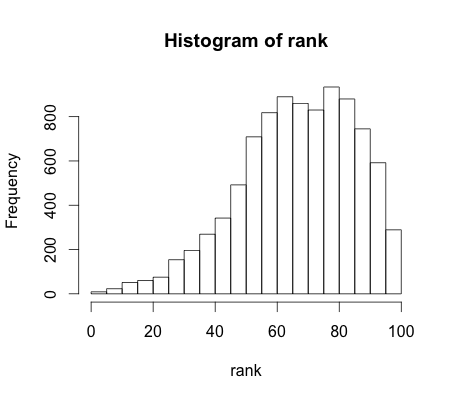
\includegraphics[scale=0.5]{Rplot01}
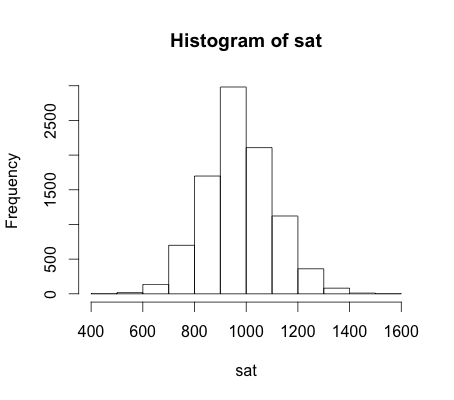
\includegraphics[scale=0.5]{Rplot}
\end{center}

In addition, calling \verb|summary()| and \verb|mean()| produces 
information about the value distribution in the vectors. 
\verb|mean()| gives the mean value for each vector. 
The values computed in this example for sat and rank were 978.21 and 67.04133 respectively.
The summary for each of the vectors is shown below.
 
\begin{figure}[H]
\begin{center}
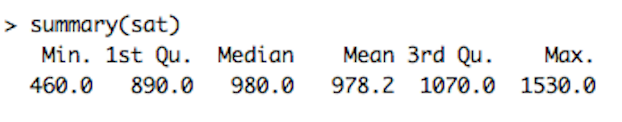
\includegraphics[scale=0.4]{satsum}
\end{center}
\caption{Summary of SAT scores}
\end{figure}

\begin{figure}[H]
\begin{center}
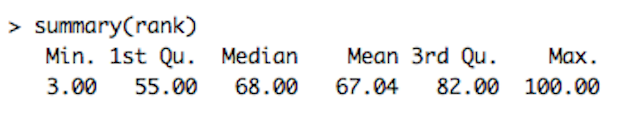
\includegraphics[scale=0.4]{ranksum}
\end{center}
\caption{Summary of student percentile rank}
\end{figure}

The values of retention are stored as 1 if the student stays until the second semester and 0 if not. 
Using the \verb|mean()| function on the vector retention gives the retention rate. 
In this case the retention rate was computed as 66.847\%. 

The retention rate is assumed correlated to the admissions requirements for SAT scores and student rank. 
The motivation for this study is to find admission requirements that maximize the 
retention rate while maintaining high enrollment. 
In order to improve admissions and retention statistics, the interrelations between these quantities should be considered. 
The relation between retention, rank and sat can be studied using yet more built in R functionality. 
A basic plot of the two is created using the command \verb|plot(rank, sat)|.

\begin{figure}[H]
\begin{center}
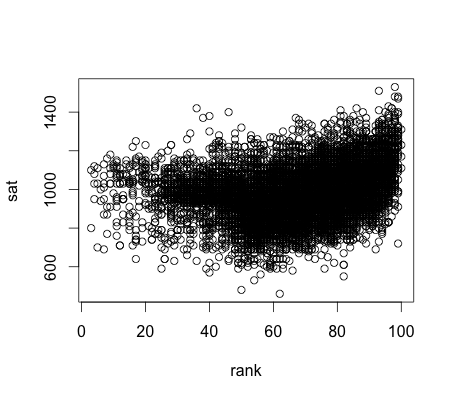
\includegraphics[scale=0.5]{Rplot02}
\end{center}
\caption{Plot of rank and sat}
\end{figure}

A plot of rank with respect to retention can be created using the plot command. 
However, since retention has values 0 and 1, R treats the vector as a quantitative variable. 
Plotting it as a factor can be done by running \verb|plot(as.factor(retention), rank)|.

\begin{figure}[H]
\begin{center}
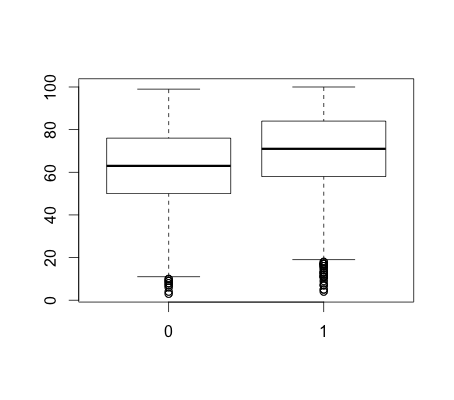
\includegraphics[scale=0.5]{Rplot03}
\end{center}
\caption{Plot of retention and rank}
\end{figure}

The \verb|lm(v1 ~ v2)| function creates a linear regression model for predicting \verb|v1| using \verb|v2|.
With this and the \verb|summary()| command which is overloaded to accept a model, the statistical significance of 
rank and sat in predicting retention can be better examined. 

The summary for \verb| summary|(lm(sat$\sim$rank)) is shown below. 
\begin{figure}[H]
\begin{center}
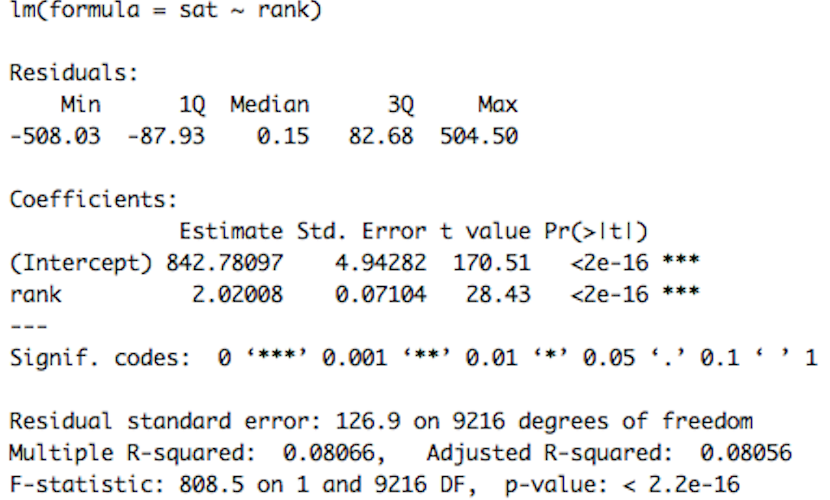
\includegraphics[scale=0.4]{ranksatlm}
\end{center}
\end{figure}

The command \verb|glm()| creates a logistic regression model. 
The summaries for the models for retention and sat and for retention and rank are shown below. 
\begin{figure}[H]
\begin{center}
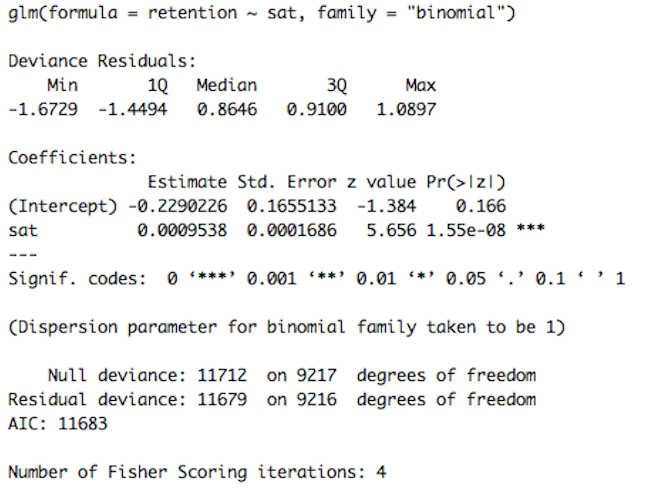
\includegraphics[scale=0.55]{retentionsat}
\end{center}
\caption{linear regression model for predicting retention with SAT score}
\end{figure}

\begin{figure}[H]
\begin{center}
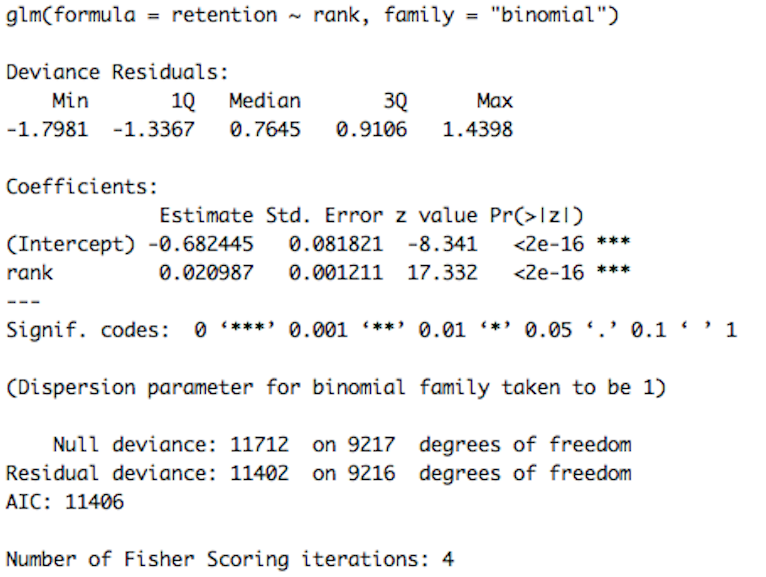
\includegraphics[scale=0.45]{retentionrankglm}
\end{center}
\caption{linear regression model for predicting retention with student rank}
\end{figure}

Finally, a logistic  regression model that predicts retention based on the combination of sat and rank is shown.

\begin{figure}[H]
\begin{center}
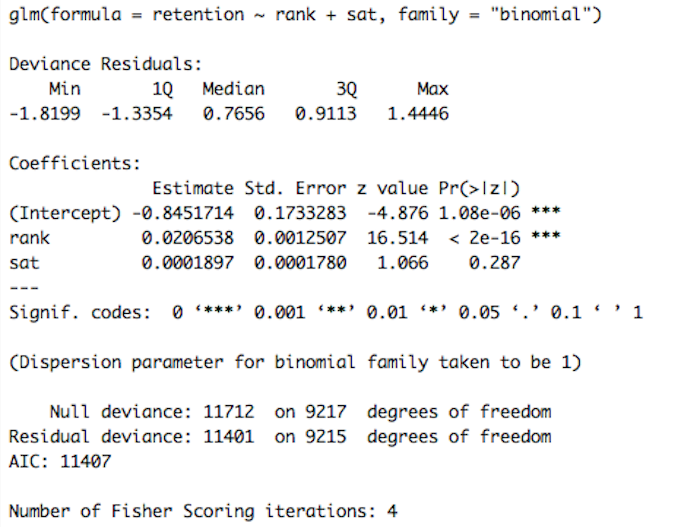
\includegraphics[scale=0.5]{retentionranksat}
\end{center}
\caption{linear regression model for predicting retention with student rank and SAT scores combined}
\end{figure}

The admissions requirements are shown in the table below. 
Those with rank over 89 are automatically admitted, so there is no SAT score 
reqirement for those with rank of 90 or above. 

\begin{center}
\begin{tabular}{|l|c|c|r|}
\hline
Percentile Rank & 1-24 & 25-49 & 50 - 89 \\ \hline
SAT Requirement & 1030 & 950 & 400 \\ \hline
\end{tabular}
\end{center}

A function was created to calculate retention rate based upon 
the admissions requirements. For the original set of requirements, the retention rate
for these requirements is 67.4\%, which is slightly higher than the retention rate with the 
admitted students. In addition, the enrollment loss (number of potential students 
not accepted based upon their rank and score) is also computed. For this set of requirements, 
547 of the 9,218 students fail to meet the requirements. Therefore the total enrollment loss is 
547. 

In order to improve retention, an alternative set of thresholds were proposed for admissions. 
Note that those with rank of 90 or above are always admitted, so the only changes are for those 
in the lower 90\% of the class. 

\begin{center}
\begin{tabular}{|l|c|c|r|}
\hline
Percentile Rank & 1-32 & 33-49 & 50 - 89 \\ \hline
SAT Requirement & 1610 & 950 & 400 \\ \hline
\end{tabular}
\end{center}

These changes resulted in a better retention rate than the previous case, and a far worse enrollment loss. 
The retention rate computed for this example is 68.1\%, while the enrollment loss is 825. 
In order to see whether there is a set of admissions thresholds that maximizes retention rate without exceeding 
the enrollment loss of 825, a brute force method was implemented that computed the enrollment loss and 
retention rate for all of the possible combinations of rank and SAT requirements. 

In order to increase efficiency for this case, I used values 1, 5, 10, ..., 85 as possible 
values for rank cutoff values and values 400, 410, ..., 1610 for SAT scores. The code for this 
project is attached. The brute force search did not result in a better retention rate than 68.1\% without 
simultaneously having an enrollment loss less than 825. 


\newpage
\begin{Verbatim}[numbers = left]
# This line replaces using the 'import dataset' option
# because I prefer writing a script over writing a 
# series of commands in console however saveable

# for this project, the dataset in FTIC.csv is an array 9128 x 6
# of stats about freshmen admitted to TSU.
# The 6 columns are TERM, QUARTER, PERCENTILE, SAT, X1st_Spring and X2nd_Fall
FTIC <- read.table("~/Dropbox/data_mining/hw01/FTIC.csv", header=TRUE, sep=",")

# pick out the 'X2nd_Fall' column from the dataset. 
# this gives the retention rate for this set of students
retention=FTIC$X2nd_Fall
# The two factors which we are going to consider as 
# predictors of retention are precentile rank and sat scores
rank=FTIC$PERCENTILE
sat=FTIC$SAT

# create histograms for rank and sat and compute
# values related to distribution for later use.
hist(rank)
summary(rank)
mean(rank)
hist(sat)
summary(sat)
mean(sat)

#make retention boolean
retention=(retention=="Y")*1

#linear regression of sat and rank
model=lm(sat~rank)
summary(model)

plot(as.factor(retention), rank)

rankmodel=glm(retention~rank, family='binomial')
summary(rankmodel)

satmodel=glm(retention~sat, family='binomial')
summary(satmodel)

model=glm(retention~rank+sat, family='binomial')
summary(model)

index = ( (rank < 25)  & (sat >= 1030) )| 
        ( (rank >= 25) & (rank < 50) & (sat >= 950) ) | 
        ( (rank >= 50) & (rank < 90) & (sat >= 400) ) |
        (rank >= 90)
table(index)
retention[index]
mean(retention[index])


# fun example of a function with a list
mysumanddiff=function(x, y){
 L = list(sum = x + y, diff = x - y)
 return(L)
}

mylist=mysumanddiff(8, 3)

mylist$sum
mylist$diff

# this function evaluates retention based on threshold requirements
# for sat and rank that are passed in. Return value is a list that
# contains enrollment loss and retention rate based on sat and rank
evalthresholds=function(rank, sat, retention, rankthresholds, 
                        satthresholds){
#index[i] = 1 if student [i] fulfills admission requirements
  index=( (rank<rankthresholds[1]) & 
          (sat>=satthresholds[1]) ) | 
        ( (rank>=rankthresholds[1]) & 
          (rank<rankthresholds[2]) & 
          (sat>=satthresholds[2]) ) |
        ( (rank>=rankthresholds[2]) & 
          (rank<rankthresholds[3]) & 
          (sat>=satthresholds[3]) ) |
        ( (rank>=rankthresholds[3]) )

  x1 = sum( (index==FALSE)*1)
  x2 = mean(retention[index])
  L = list(enrollmentloss = x1, newretention = x2)
  return(L)
}
# test this function with solution in homework to see if it works.
rankthresholds=c(25,50)
satthresholds=c(1030,950,400)
mylist=evalthresholds(rank,sat,retention,rankthresholds,satthresholds)
mylist$enrollmentloss
mylist$newretention

# now compute enrollmentloss and retention 
# with a different set of threshold criteria
rankthresholds=c(33,50, 90)
satthresholds=c(1610,950,400)

mylist=evalthresholds(rank,sat,retention,rankthresholds,satthresholds)
mylist$enrollmentloss
mylist$newretention

finalrankthreshold=rankthresholds
finalsatthreshold=satthresholds

# brute force method to compute better possible threshold requirements
# for admissions based on sat and rank
for(i in 10:78){
  for(j in 20:89){
    if(i < j){
      print(paste(i,j))
      rankthresholds=c(i,j,90)
      for(k in 95:160){
        print(k)
        kk = 10*k
        for(m in 50:95){
          mm = 10*m
          for(n in 40:50){
            nn = 10*n
            satthresholds=c(nn, mm, kk)
            newlist = evalthresholds(rank,sat,retention,rankthresholds,satthresholds)
            if( (newlist$enrollmentloss<=mylist$enrollmentloss) & 
                (newlist$newretention>mylist$newretention)){
                mylist=newlist
                finalrankthreshold=rankthresholds
                finalsatthreshold=satthresholds
                print(paste("changed values", i,j,k,m,n))
            }
          }
        }
      }
    }
  }
}
print("==============================================")
print("=========Final Enrollment Statistics==========")
print("==============================================")
print(paste("Enrollment loss:",mylist$enrollmentloss))
print(paste("Enrollment loss:",mylist$newretention))

print("The final rank thresholds are: ")
print(finalrankthreshold)
print(finalsatthreshold)

#expand.grid(1:5,10:13)
\end{Verbatim}

\end{document}
